%\documentclass[preprint,tightenlines,showpacs,showkeys,floatfix,
%nofootinbib,superscriptaddress,fleqn]{revtex4} 
\documentclass[tightenlines,floatfix,nofootinbib,superscriptaddress,fleqn]{revtex4-2} 
%\documentclass[aps,epsfig,tightlines,fleqn]{revtex4}
\usepackage{kotex}
\usepackage[HWP]{dhucs-interword}
\usepackage[dvips]{color}
\usepackage{graphicx}
\usepackage{bm}
%\usepackage{fancyhdr}
%\usepackage{dcolumn}
\usepackage{defcolor}
\usepackage{amsmath}
\usepackage{amsfonts}
\usepackage{amssymb}
\usepackage{amscd}
\usepackage{amsthm}
\usepackage[utf8]{inputenc}
%\pagestyle{fancy}

\begin{document}

\title{\Large 2022년 2학기 물리학 II}
\author{김현철\footnote{Office: 5S-436D (면담시간 매주
    수요일-16:15$\sim$19:00)}} 
\email{hchkim@inha.ac.kr}
\affiliation{Hadron Theory Group, Department of Physics,
  Inha  University, Incheon 22212, Republic of Korea }
\date{Autumn Semester, 2022}
\author{Hui-Jae Lee} 
\email{hjlee6674@inha.edu}
\affiliation{Hadron Theory Group, Department of Physics,
  Inha  University, Incheon 22212, Republic of Korea }
\date{Autumn Semester, 2022}
\maketitle


\section*{\large Quiz 13}
\noindent {\bf 문제 1 [20pt]}
빛이 물의 표면에 $53.0^\circ$로 입사하였다. 물의 굴절률이 1.33일 때, 물
내부로 굴절된 빛의 굴절각은 얼마인가? 또 입사각과 굴절각의 합은
얼마인가? 이 경우 물의 표면에서 반사된 빛은 한 방향으로 편광되어
있음을 증명하여라. 

\noindent {\bf 풀이 : }
물의 표면에 입사각 $53.0^\circ$로 입사하였고 물의 굴절률이 1.33이므로 스넬의 법칙에 의해
굴절각 $\theta$는
\begin{align}
  \sin 53.0^\circ = 1.33\sin\theta \Longrightarrow
  \theta = \arcsin\left(\frac{\sin 53.0^\circ}{1.33}\right)=36.9^\circ
\end{align}
$36.9^\circ$이고 입사각과 굴절각의 합은 $53.0^\circ+36.9^\circ\approx 90^\circ$이다.
반사각은 입사각과 같으므로 반사각과 굴절각의 합이 $90^\circ$이다. 물의 브루스터 각 $\theta_B$는
\begin{align}
  \theta_B = \arctan\left(\frac{1.33}{1}\right)
  =53.1^\circ
\end{align}
로 반사각과 거의 일치한다. 따라서 물의 표면에서 반사된 빛은 한 방향으로 편광되어 있다.
\vspace{1cm}

\noindent {\bf 문제 2 [20pt]}
곡률반지름이 20.0 cm인 볼록거울의 축상에서 14.0 cm 앞부분에 점광원이
놓여 있다면 상이 생기는 지점은 어디인가? 이 상은 실상인가 아니면 허상인가?

\noindent {\bf 풀이 : }
볼록거울의 거울공식은
\begin{align}
  \frac{1}{p} + \frac{1}{q} = \frac{2}{R}
\end{align}
이다. $p$는 점광원과 거울 사이 거리, $q$는 상이 맺히는 지점과 거울 사이 거리, 
$R$은 곡률 반지름이다. 볼록 거울이므로 $R =-$20.0 cm이고 $p=$14.0 cm이다. 따라서 $q$는
\begin{align}
  \frac{1}{q} = -\frac{1}{14.0~\mathrm{cm}} -\frac{1}{20.0~\mathrm{cm}}
  = -\frac{34.0}{280~\mathrm{cm}} \Longrightarrow
  q = -\frac{280~\mathrm{cm}}{34.0} = -8.24~\mathrm{cm}
\end{align}
이다. 즉, 상은 거울 뒤 8.24 cm 지점에 생기고 허상이다.
\vspace{1cm}


\noindent {\bf 문제 3 [50pt]}
그림~\ref{fig:1}에서 직각 모서리 프리즘 (corner cube prism) 2개의 거울을
직각으로 붙여 만든 그릇에 물을 담은 형태를 생각하자. 빛이 수면에
수직으로 입사하는 경우, 빛은 물을 지나 1개의 거울면에서 반사하고 다시
다른 거울면에서 반사하여 물을 빠져나올 것이다.
% \begin{figure}[htp]
%   \centering
%   \includegraphics[scale=0.5]{qfig14-1.png}
%   \caption{\textbf{문제 3}}
%   \label{fig:1}
% \end{figure}
\begin{itemize}
\item[(가)] 이때 두 번 반사된 빛은 원래의 입사광과 평행하게 되돌아가게
  된다는 것을 증명하여라.
\item[(나)] 빛이 비스듬하게 입사하는 경우에도 반사된 빛은 항상 입사한
  빛에 평행이 된다는 것을 증명하여라.
\item[(다)] 정육면체 유리 덩어리의 모서리를 45° 각도로 잘라내어
  만들어진 피라미드 형태의 유리에 대 해서도 위의 관계가 성립되는 것을
  보여라. 이 때 유리의 굴절률이 1.45라고 가정하고 전반사 조건을
  고려하여라. 실제로, 사고 예방을 위해서 자전거 등에는 밤에 다른
  자동차의 불빛에 의해 빛나게 되는 물체를 부착하는데, 이 물체는 이 와
  같은 작은 피라미드 모양의 플라스틱을 여러 개 붙여 놓은
  형태이다. 자동차 양끝의 방향지 시등 커버도 이와 같이 되어 있다.  
\end{itemize}

\noindent {\bf 풀이 : }
먼저 빛이 입사각 $\theta_1$를 가지고 입사한다고 해보자. 공기의 굴절률을 $n_1$,
물의 굴절률을 $n_2$라 하면 스넬의 법칙에 의해
\begin{align}\label{eq:3-1}
  n_1\sin\theta_1 = n_2\sin\theta_2
\end{align}
이다. $\theta_2$는 굴절각이다. $\theta_2$ 만큼의 굴절각을 가지고 
시계 방향으로 $\pi/4$만큼 기울어진 거울에 반사되면 $\pi/4+\theta_2$ 만큼의 반사각을
가지게 되고 다시 반시계 방향으로 $\pi/4$만큼 기울어진 거울에 반사되면 $\pi/4-\theta_2$
만큼의 반사각을 가지고 반사된다. 이 빛은 수면에 대해 $\theta_2$의 입사각을 가지고
입사하게 되어 다시 스넬의 법칙에 의해 $\theta_1$의 굴절각으로 프리즘을 빠져나온다.
\begin{itemize}
  \item[(가)]
  빛이 수직으로 입사하는 경우는 $\theta_1=0^\circ$이고 마지막에 빠져나온 빛 또한 굴절각
  $\theta_1=0^\circ$을 가진다. 두 빛 모두 수면에 수직이므로 두번 반사된 빛과 입사광은
  평행하다.
  \item[(나)]
  빛이 비스듬하게 입사하면 $\theta_1\neq 0$이고 위의 서술에 의해 반사되어 빠져나온 빛 또한
  $\theta_1$의 굴절각을 가지고 빠져나온다. 두 빛이 수면과 이루는 각도가 같으므로 두 빛은
  평행하다.
  \item[(다)] 
  굴절률이 1.45인 유리에서 공기로 빛이 빠져나갈 때 유리의 표면에서 빛이 전반사되는
  입사각 $\theta_c$를 다음과 같이 구할 수 있다.
  \begin{align}
    1.45\sin\theta_c = \sin90^\circ\Longrightarrow
    \theta_c = \arcsin\left(\frac{1}{1.45}\right)\approx 43.6^\circ.
  \end{align}
  따라서 거울에 빛이 반사될 때 반사각은 항상 $\theta_c$보다 커야 한다.
  빛이 전반사되어야 하는 경우는 총 두 경우인데 각각 빛의 입사각은 
  $\pi/4+\theta_2$와 $\pi/4-\theta_2$이다. $\theta_2$는 식~\eqref{eq:3-1}에 의해
  \begin{align}
    \sin\theta_1 = 1.45\sin\theta_2\Longrightarrow
    \theta_2 = \arcsin\left(\frac{\sin\theta_1}{1.45}\right)
  \end{align}
  로 쓸 수 있으므로 반사되어야 하는 표면에 대한 빛의 두 입사각 $\phi_1$, $\phi_2$를
  \begin{align}
    \begin{split}
      \phi_1 &= \frac{\pi}{4}+\theta_2 = \frac{\pi}{4}
      +\arcsin\left(\frac{\sin\theta_1}{1.45}\right), \\
      \phi_2 &= \frac{\pi}{4}-\theta_2 = \frac{\pi}{4}
      -\arcsin\left(\frac{\sin\theta_1}{1.45}\right)
    \end{split}
  \end{align}
  와 같이 쓸 수 있다. 먼저 $\phi_1$가 $\theta_c$보다 커야 하므로
  $0<\phi_1<\pi/2$ 이므로 
  \begin{align}
    \phi_1 = \frac{\pi}{4}
    +\arcsin\left(\frac{\sin\theta_1}{1.45}\right)
    >43.6^\circ \Longrightarrow
    \sin\theta_1>0>-1.45\sin1.4^\circ
  \end{align}
  이고 처음 입사각 $\theta_1$가 $0<\theta_1<\pi/4$를 만족해야 첫번째 전반사면에
  도달하므로 $\phi_1$의 전반사 조건에 의한 $\theta_1$의 범위는
  $0<\theta_1<\pi/4$이다. $\phi_2$ 또한 $\theta_c$보다 커야한다는 사실을 이용해
  \begin{align}
    \begin{split}
      \phi_2 =  \frac{\pi}{4}
      -\arcsin\left(\frac{\sin\theta_1}{1.45}\right)
      >43.6^\circ &\Longrightarrow
      \sin\theta_1<1.45\sin1.4^\circ = 0.354 \\
      &\Longrightarrow\theta_1 < 2.03^\circ
    \end{split}
  \end{align}
  $\theta_1$가 $2.03^\circ$보다 작아야 함을 알 수 있다. 따라서 입사한 빛이 유리에 입사하여
  두번 전반사되기 위해 필요한 입사각 $\theta_1$의 조건은 $0^\circ\leq \theta_1
  <2.03^\circ$이다.
\end{itemize}
 

\vspace{1cm}


\noindent {\bf 문제 4 [100pt] {\color{red} (난이도 상)}} 
그림~\ref{fig:2}에서는 수영장 수면 위 $d_1=250$ cm 위에 매달려 있는
작은 전구를 보여준다. 수영장의 깊이는 $d_2=200$ cm이다. 수영장
바각에는 큰 거울이 놓여 있다. 이 전구의 상은 수면에서부터 밑으로 얼마나 멀리
놓여 있는가? 
\begin{figure}[htp]
  \centering
  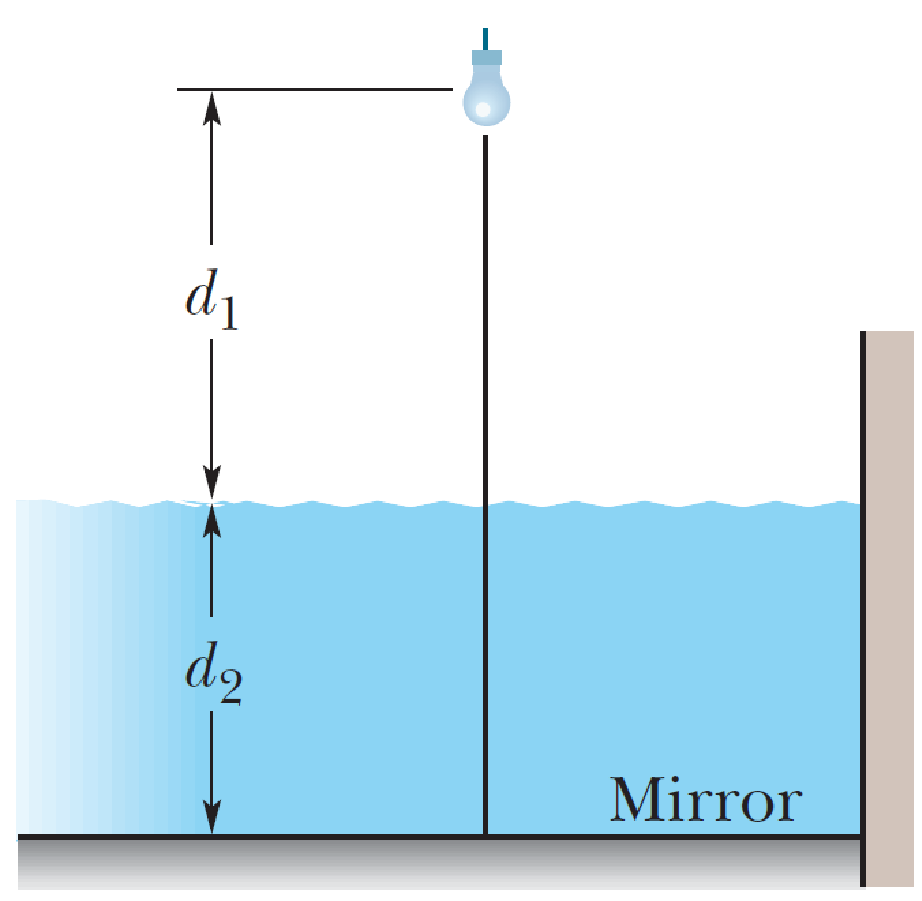
\includegraphics[scale=0.35]{qfig13-4-20221031.pdf} 
  \caption{\textbf{문제 4}}
  \label{fig:2}
\end{figure}

\begin{itemize}
\item \noindent 귀띔 1: 빛살(ray)는 전구를 지나는 수직축에 가까이 있다고
가정하여라. 그러면 $\sin\theta\approx \tan\theta \approx \theta$와
같은 근사를 쓸 수 있다.
\item \noindent 귀띔 2: 다음 그림~\ref{fig:3}을 참조해서 문제를 푸세요.
\end{itemize}
\begin{figure}[htp]
  \centering
  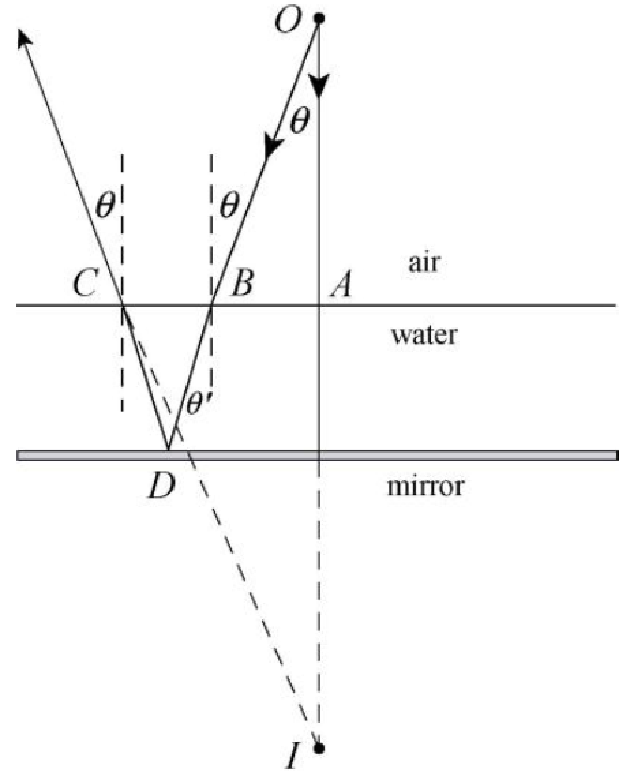
\includegraphics[scale=0.5]{qfig13-4-1-20221031.pdf} 
  \caption{\textbf{문제 4 귀띔}}
  \label{fig:3}
\end{figure}



\noindent {\bf 풀이 : }
수면으로부터 전구의 상 까지의 거리 $\overline{AI}$를 구하기 위해 삼각비를 이용하자.
수면과 거울이 평행이고 $\overline{CI}$는
거울에서 반사되어 공기 중에서 진행 중인 빛의 연장선이므로 각 $\angle AIC$의 크기는 $\theta$이다.
또한 $\overline{CA}$와 $\overline{AI}$는 수직이므로 
각  $\angle AIC$에 대한 $\tan$ 값은
\begin{align}
  \tan(\angle AIC) = \tan\theta = \frac{\overline{CA}}{\overline{AI}}
\end{align}
이고 이로부터
\begin{align}\label{eq:4-1}
  \overline{AI} = \frac{\overline{CA}}{\tan\theta}
\end{align}
이다. 다시 $\overline{CA} =\overline{CB}+\overline{BA} $이고
$\overline{CB}$와 $\overline{BA}$는 각각
\begin{align}
  \overline{CB} = 2d_2\tan\theta',\,\,\,
  \overline{BA} = d_1\tan\theta
\end{align}
이므로 식~\eqref{eq:4-1}에 대입하여
\begin{align}\label{eq:4-2}
  \overline{AI} = \frac{d_1\tan\theta+2d_2\tan\theta'}{\tan\theta}
  =d_1+2d_2\frac{\tan\theta'}{\tan\theta}
\end{align}
를 얻는다. 여기서 근사 $\tan\theta\approx\sin\theta$를 이용하면
\begin{align}
  \frac{\tan\theta'}{\tan\theta}\approx
  \frac{\sin\theta'}{\sin\theta}
\end{align}
이고 스넬의 법칙을 이용하면
\begin{align}
  n_1\sin\theta=n_2\sin\theta'
\end{align}
이다. $n_1$은 공기의 굴절률이고 $n_2$는 물의 굴절률이다. 따라서 $\tan$의 비를
\begin{align}
  \frac{\tan\theta'}{\tan\theta}\approx\frac{n_1}{n_2}
  =\frac{1}{n_2}
\end{align}
로 얻을 수 있고 식~\eqref{eq:4-2}에 대입하여
\begin{align}
  \overline{AI} =d_1+\frac{2d_2}{n_2}
\end{align}
$\overline{AI}$를 구할 수 있다.
\begin{align}
  \overline{AI} =250~\mathrm{cm}+\frac{2(200~\mathrm{cm})}{1.33}
  =551~\mathrm{cm}.
\end{align}
따라서 전구의 상은 수면에서부터 551 cm 아래에 생긴다.
\vspace{1cm}


\end{document}

